\subsection{Dilepton studies in CR4}
\label{sec:cr4}

\subsubsection{Modeling of Additional Hard Jets in Top Dilepton Events}
\label{sec:jetmultiplicity}

Dilepton \ttbar\ events have 2 jets from the top decays, so additional
jets from radiation or higher order contributions are required to
enter the signal sample.   In this Section we develop an algorithm
to be applied to all \ttll\ MC samples to insure that the distribution
of extra jets is properly modelled.


The modeling of additional jets in \ttbar\
events is checked in a \ttll\ control sample,
selected by requiring
\begin{itemize}
\item exactly 2 selected electrons or muons with \pt $>$ 20 GeV
\item \met\ $>$ 50 GeV
\item $\geq1$ b-tagged jet
\item Z-veto ($|m_{\ell\ell} - 91| > 15$ GeV)
\end{itemize}
Figure~\ref{fig:dileptonnjets} shows a comparison of the jet
multiplicity distribution in data and MC for this two-lepton control
sample. After requiring at least 1 b-tagged jet, most of the
events have 2 jets, as expected from the dominant process \ttll. There is also a
significant fraction of events with additional jets. 
The 3-jet sample is mainly comprised of \ttbar\ events with 1 additional
emission and similarly the $\ge4$-jet sample contains primarily
$\ttbar+\ge2$ jet events. 
%Even though the primary \ttbar\
%Madgraph sample used includes up to 3 additional partons at the Matrix
%Element level, which are intended to describe additional hard jets,
%Figure~\ref{fig:dileptonnjets} shows a slight mis-modeling of the
%additional jets. 


\begin{figure}[hbt]
  \begin{center}
	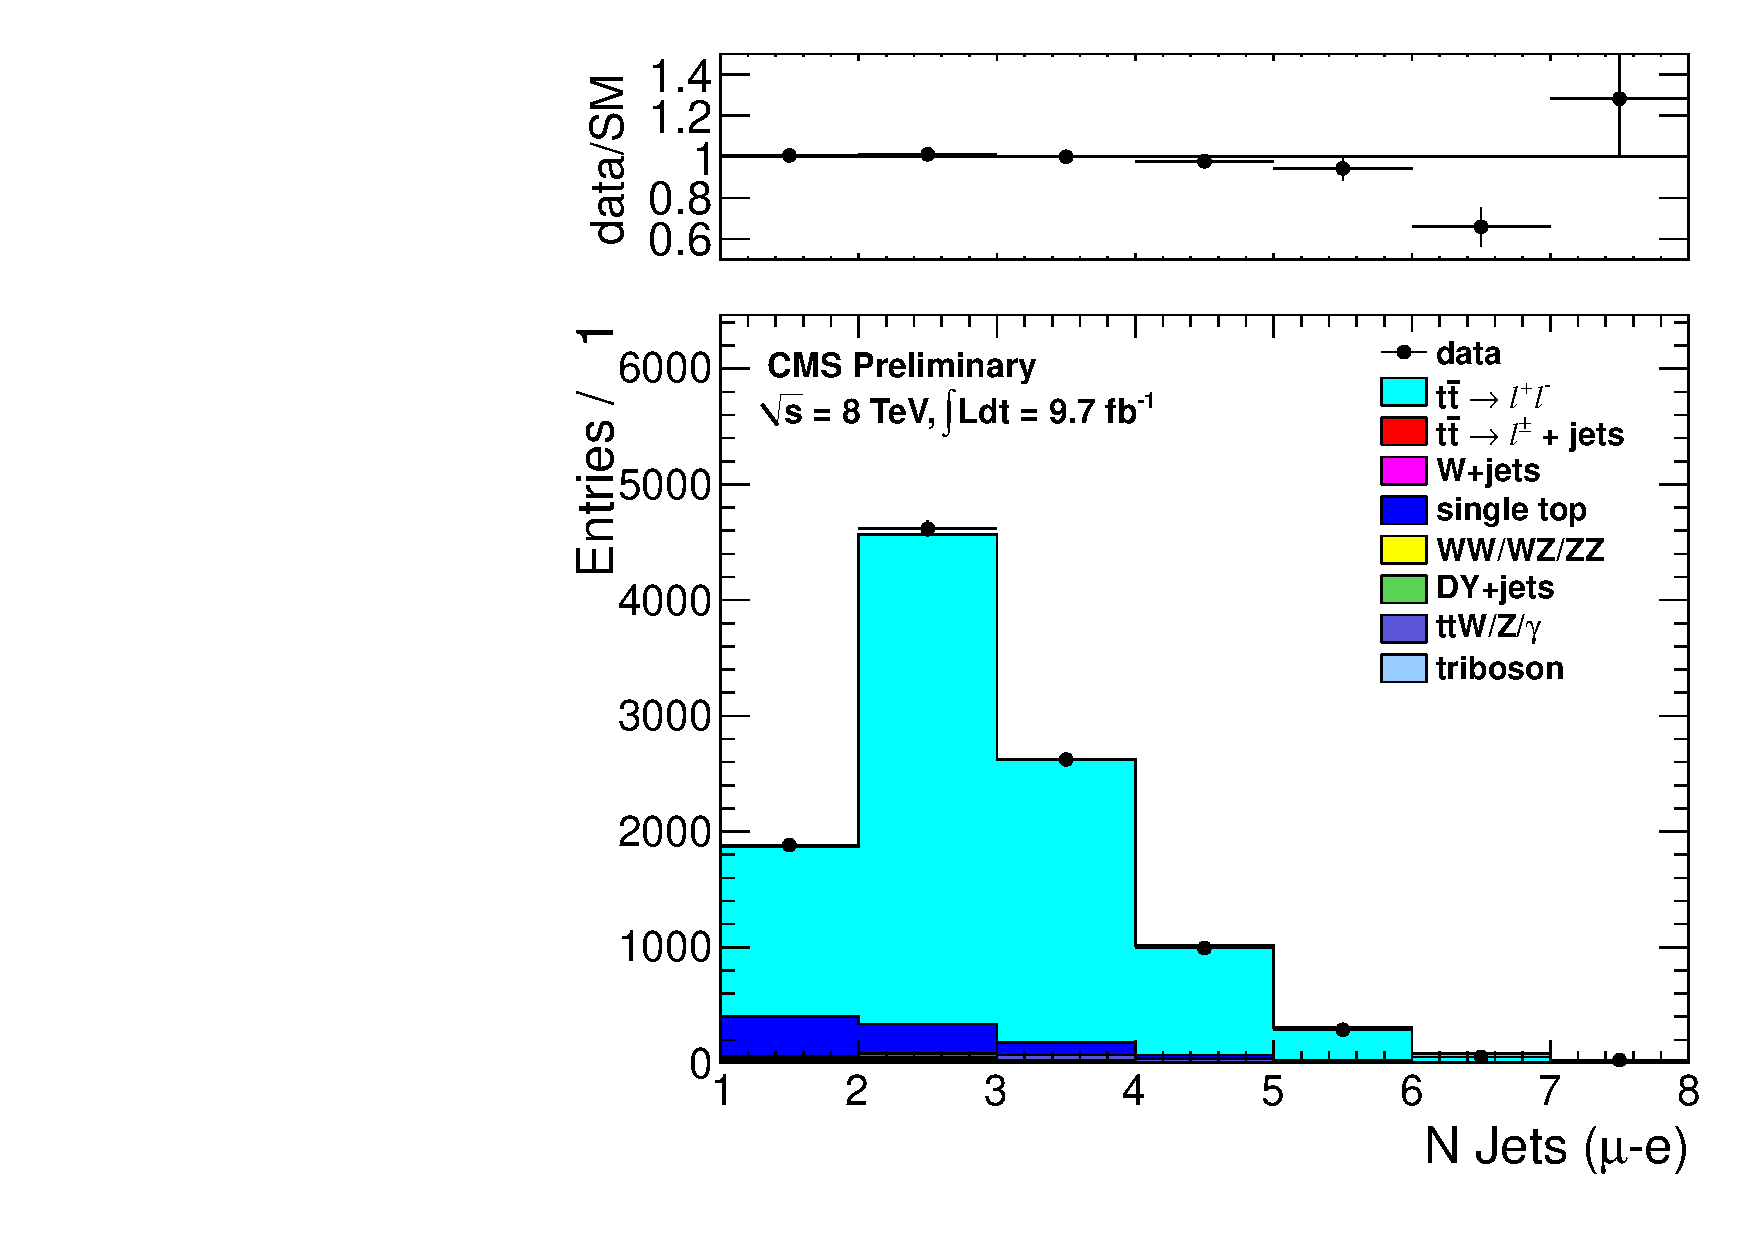
\includegraphics[width=0.5\linewidth]{plots/njets_all_met50_mueg.pdf}
	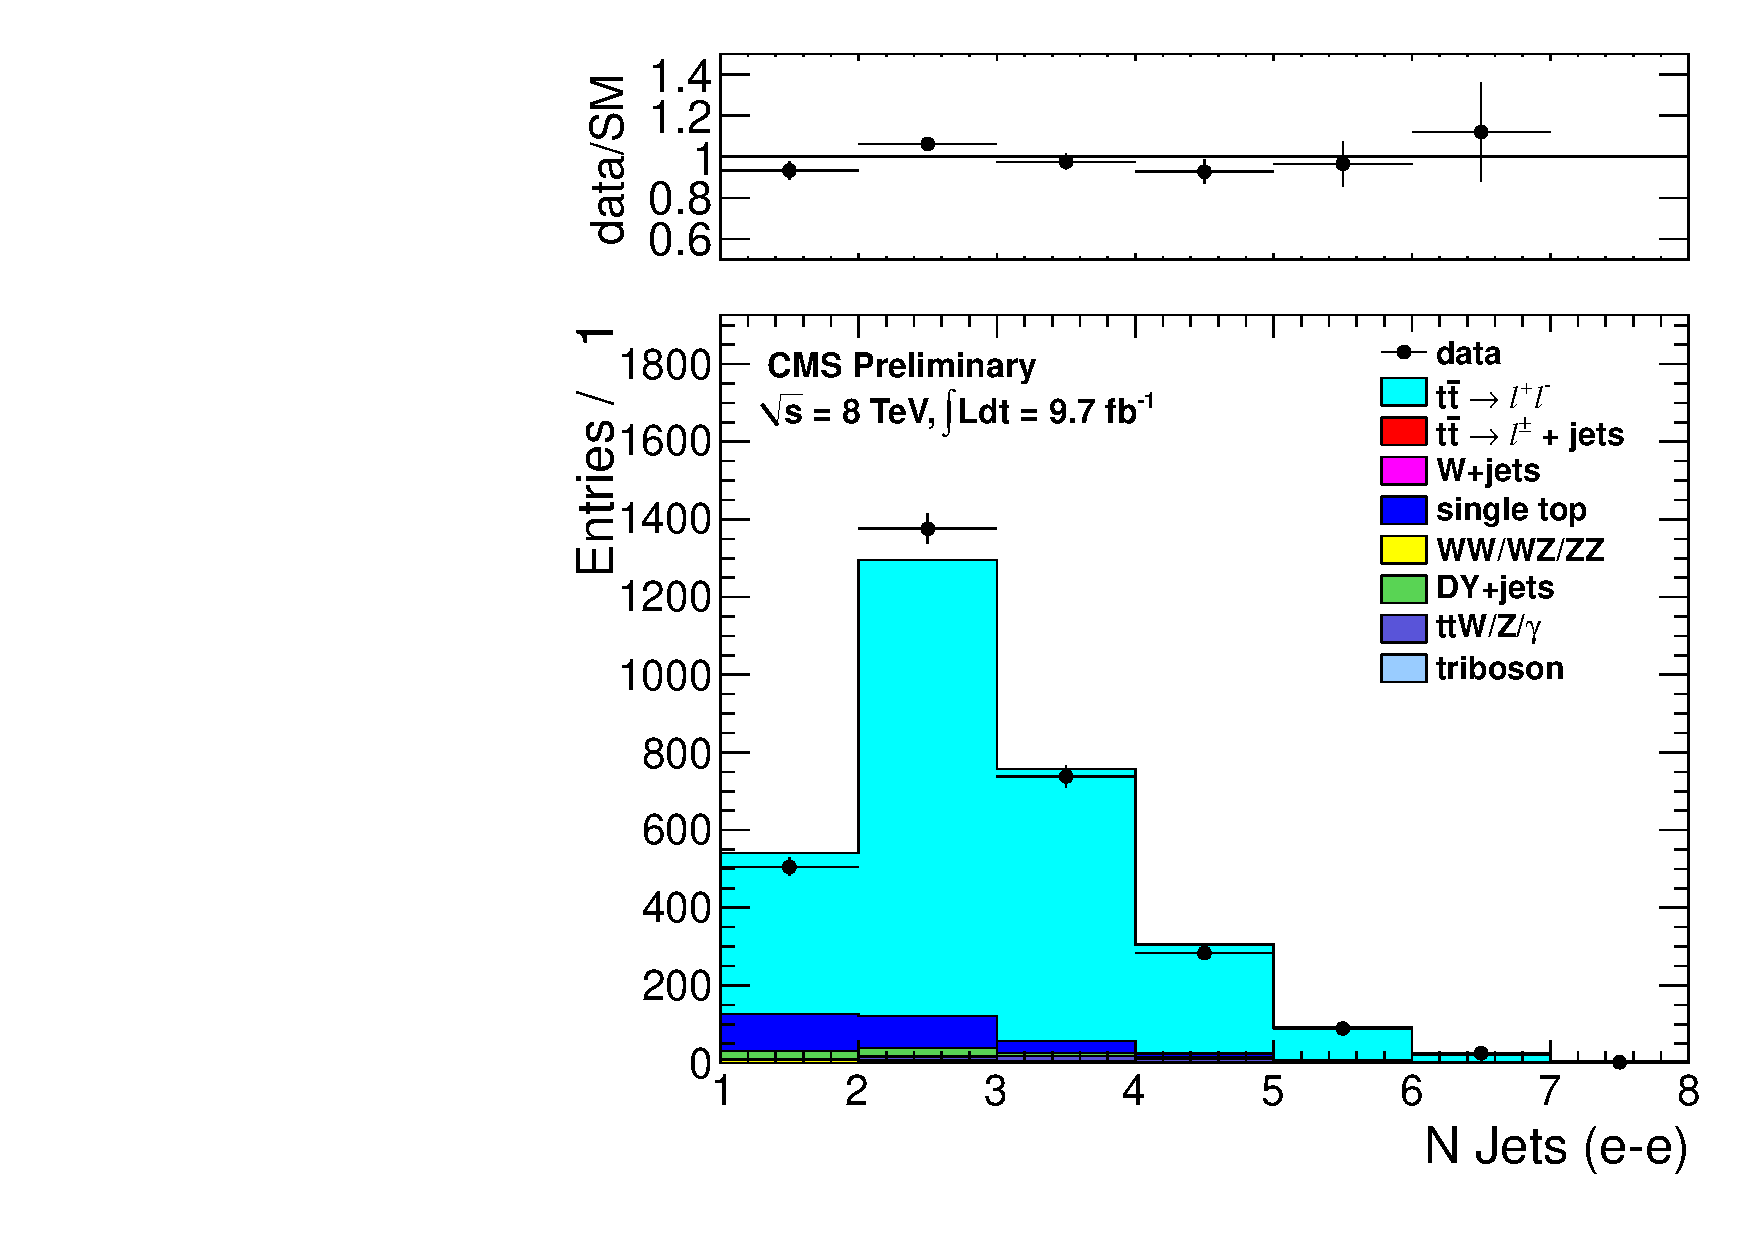
\includegraphics[width=0.5\linewidth]{plots/njets_all_met50_diel.pdf}%
        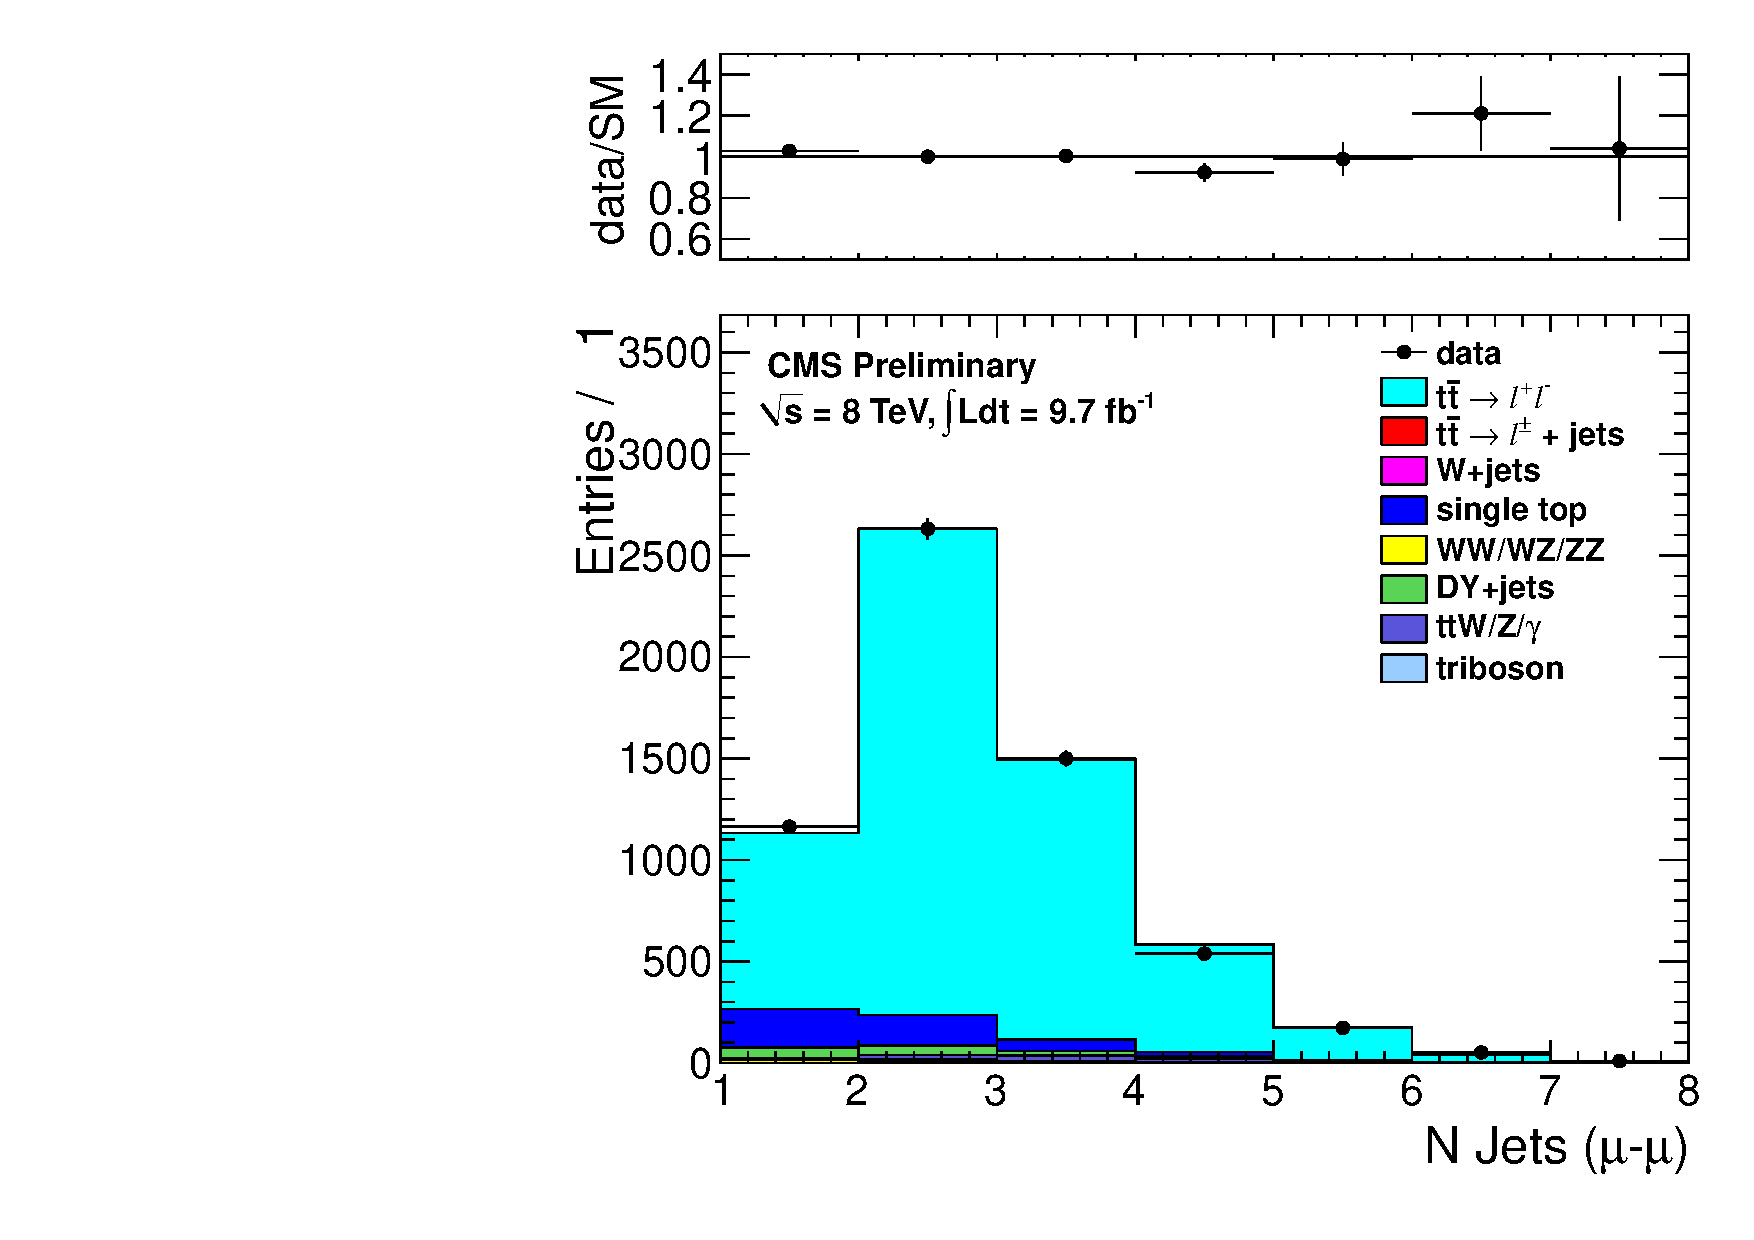
\includegraphics[width=0.5\linewidth]{plots/njets_all_met50_dimu.pdf}
	\caption{
	  \label{fig:dileptonnjets}%\protect 
          Comparison of the jet multiplicity distribution in data and MC for dilepton events in the \E-\M\
          (top), \E-\E\ (bottom left) and \M-\M\ (bottom right) channels.}  
      \end{center}
\end{figure}

It should be noted that in the case of \ttll\ events
with a single reconstructed lepton, the other lepton may be
mis-reconstructed as a jet. For example, a hadronic tau may be
mis-identified as a jet (since no $\tau$ identification is used). 
In this case only 1 additional jet from radiation may suffice for 
a \ttll\ event to enter the signal sample. As a result, both the
samples with $\ttbar+1$ jet and $\ttbar+\ge2$ jets are relevant for
estimating the top dilepton background in the signal region.

%In this section we discuss a correction to $ N_{2 lep}^{MC} $ in Equation XXX
%due to differences in the modelling of the jet multiplicity in data versus MC.
%The same correction also enters $ N_{peak}^{MC}$ in Equation XXX to the extend that the 
%dilepton contributions to $ N_{peak}^{MC}$ gets corrected.

%The dilepton control sample is defined by the following requirements:
%\begin{itemize}
%\item Exactly 2 selected electrons or muons with \pt $>$ 20 GeV
%\item \met\ $>$ 50 GeV
%\item $\geq1$ b-tagged jet
%\end{itemize}
%
%This sample is dominated by \ttll. The distribution of \njets\ for data and MC passing this selection is displayed in Fig.~\ref{fig:dilepton_njets}. 
%We use this distribution to derive scale factors which reweight the \ttll\ MC \njets\ distribution to match the data. We define the following
%quantities
%
%\begin{itemize}
%\item $N_{2}=$ data yield minus non-dilepton \ttbar\ MC yield for \njets\ $\leq$ 2
%\item $N_{3}=$ data yield minus non-dilepton \ttbar\ MC yield for \njets\ = 3
%\item $N_{4}=$ data yield minus non-dilepton \ttbar\ MC yield for \njets\ $\geq$ 4
%\item $M_{2}=$ dilepton \ttbar\ MC yield for \njets\ $\leq$ 2
%\item $M_{3}=$ dilepton \ttbar\ MC yield for \njets\ = 3
%\item $M_{4}=$ dilepton \ttbar\ MC yield for \njets\ $\geq$ 4
%\end{itemize}
%
%We use these yields to define 3 scale factors, which quantify the data/MC ratio in the 3 \njets\ bins:
%
%\begin{itemize}
%\item $SF_2 = N_2 / M_2$
%\item $SF_3 = N_3 / M_3$
%\item $SF_4 = N_4 / M_4$
%\end{itemize}
%
%And finally, we define the scale factors $K_3$ and $K_4$:
%
%\begin{itemize}
%\item $K_3 = SF_3 / SF_2$
%\item $K_4 = SF_4 / SF_2$
%\end{itemize}
%
%The scale factor $K_3$ is extracted from dilepton \ttbar\ events with \njets = 3, which have exactly 1 ISR jet.
%The scale factor $K_4$ is extracted from dilepton \ttbar\ events with \njets $\geq$ 4, which have at least 2 ISR jets.
%Both of these scale factors are needed since dilepton \ttbar\ events which fall in our signal region (including
%the \njets $\geq$ 4 requirement) may require exactly 1 ISR jet, in the case that the second lepton is reconstructed
%as a jet, or at least 2 ISR jets, in the case that the second lepton is not reconstructed as a jet. These scale
%factors are applied to the dilepton \ttbar\ MC only. For a given MC event, we determine whether to use $K_3$ or $K_4$
%by counting the number of reconstructed jets in the event ($N_{\rm{jets}}^R$) , and subtracting off any reconstructed 
%jet which is matched to the second lepton at generator level ($N_{\rm{jets}}^\ell$); $N_{\rm{jets}}^{\rm{cor}} = N_{\rm{jets}}^R - N_{\rm{jets}}^\ell$.
%For events with $N_{\rm{jets}}^{\rm{cor}}=3$ the factor $K_3$ is applied, while for events with $N_{\rm{jets}}^{\rm{cor}}\geq4$ the factor $K_4$ is applied.
%For all subsequent steps, the scale factors $K_3$ and $K_4$ have been
%applied to the \ttll\ MC.


Table~\ref{tab:njetskfactors}  shows scale factors ($K_3$ and $K_4$)
used to correct the
fraction of events with additional jets in MC to the observed fraction
in data.   These scale factors are calculated from Fig.~\ref{fig:dileptonnjets} 
as follows:
\begin{itemize}
\item $N_{2}=$ data yield minus non-dilepton \ttbar\ MC yield for
  \njets\ =1 or 2.
\item $N_{3}=$ data yield minus non-dilepton \ttbar\ MC yield for \njets\ = 3
\item $N_{4}=$ data yield minus non-dilepton \ttbar\ MC yield for \njets\ $\geq$ 4
\item $M_{2}=$ dilepton \ttbar\ MC yield for \njets\ = 1 or 2
\item $M_{3}=$ dilepton \ttbar\ MC yield for \njets\ = 3
\item $M_{4}=$ dilepton \ttbar\ MC yield for \njets\ $\geq$ 4
\end{itemize}
\noindent then
\begin{itemize}
\item $SF_2 = N_2 / M_2$
\item $SF_3 = N_3 / M_3$
\item $SF_4 = N_4 / M_4$
\item $K_3 = SF_3 / SF_2$
\item $K_4 = SF_4 / SF_2$
\end{itemize}
\noindent This insures that $K_3 M_3/(M_2 + K_3 M_3 + K_4 M_4) = N_3 /
(N_2+N_3+N_4)$ and similarly for the $\geq 4$ jet bin.

Table~\ref{tab:njetskfactors} also shows the values of $K_3$ and $K_4$ when the \met\ cut in the control sample definition is changed from 50 GeV to 100 GeV and 150 GeV.
% These values of $K_3$ and $K_4$ are not used in the analysis, but 
This demonstrate that there is no statistically significant dependence of $K_3$ and $K_4$ on the \met\ cut.


The factors $K_3$ and $K_4$ (derived with the 100 GeV \met\ cut) are applied to the \ttll\ MC throughout the
entire analysis, i.e. 
whenever \ttll\ MC is used to estimate or subtract
a yield or distribution.   To be explicit, whenever Powheg is used,
the Powheg $K_3$ and $K_4$ are used; whenever default MadGraph is 
used, the MadGraph $K_3$ and $K_4$ are used, etc.
%
In order to do so, it is first necessary to count the number of
additional jets from radiation and exclude leptons mis-identified as
jets. A jet is considered a mis-identified lepton if it is matched to a
generator-level second lepton with sufficient energy to satisfy the jet
\pt\ requirement ($\pt>30~\GeV$).   Then \ttll\ events that need two
radiation jets to enter our selection are scaled by $K_4$,
while those that only need one radiation jet  are scaled by $K_3$.

\begin{table}[!ht]
\begin{center}
\begin{tabular}{l|c|c|c}
\cline{2-4}
                        & \multicolumn{3}{c}{ \met\ cut for data/MC scale factors} \\
\hline
Jet Multiplicity Sample &  50 GeV & 100 GeV & 150 GeV  \\
\hline
\hline
N jets $= 3$ (sensitive to $\ttbar+1$ extra jet from radiation)
& $K_3 = 0.98 \pm 0.02$ & $K_3 = 1.01 \pm 0.03$ & $K_3 = 1.00 \pm 0.08$ \\
N jets $\ge4$ (sensitive to $\ttbar+\ge2$ extra jets from radiation)
& $K_4 = 0.94 \pm 0.02$ & $K_4 = 0.93 \pm 0.04$ & $K_4 = 1.00 \pm 0.08$ \\
\hline
\end{tabular}
\caption{Data/MC scale factors used to account for differences in the
  fraction of events with additional hard jets from radiation in
  \ttll\ events. The values derived with the 100 GeV \met\ cut are applied 
  to the \ttll\ MC throughout the analysis. \label{tab:njetskfactors}}
\end{center}
\end{table}

\clearpage



\subsubsection{Validation of the ``Physics'' Modelling of the \ttdl\
  MC in CR4}
\label{sec:CR4-valid}

As mentioned above, $t\bar{t} \to $ dileptons where one of the leptons
is somehow lost constitutes the main background.
The object of this test is to validate the $M_T$ distribution of this
background by looking at the $M_T$ distribution of well identified
dilepton events.
We construct a transverse mass variable from the leading lepton and
the \met.  We distinguish between events with leading electrons and
leading muons.  

The $t\bar{t}$ MC is corrected using the $K_3$ and $K_4$ factors
from Section~\ref{sec:jetmultiplicity}.  It is also normalized to the 
total data yield separately for the \met\ requirements of signal
regions A, B, C, and D.  These normalization factors are listed
in Table~\ref{tab:cr4mtsf} and are close to unity.

The underlying \met\ and $M_T$ distributions are shown in 
Figures~\ref{fig:cr4met} and~\ref{fig:cr4mtrest}.  The data-MC agreement
is quite good.  Quantitatively, this is also shown in Table~\ref{tab:cr4yields}.
This is a {\bf very} important Table.  It shows that for well
identified \ttdl\ , the MC can predict the $M_T$ tail.  Since the
main background is also \ttdl\ except with one ``missed'' lepton, 
this is a key test.

\begin{table}[!h]
\begin{center}
{\footnotesize
\begin{tabular}{l||c||c|c|c|c|c|c}
\hline
Sample              & CR4PRESEL & CR4A & CR4B & CR4C &
CR4D & CR4E & CR4F\\
\hline
\hline
$\mu$ Data/MC-SF 	  & $1.01 \pm 0.03$ & $0.96 \pm 0.04$ & $0.99 \pm 0.07$ & $1.05 \pm 0.13$ & $0.91 \pm 0.20$ & $1.10 \pm 0.34$ & $1.50 \pm 0.67$ \\
\hline
\hline
e Data/MC-SF 	  & $0.99 \pm 0.03$ & $0.99 \pm 0.05$ & $0.91 \pm 0.08$ & $0.84 \pm 0.13$ & $0.70 \pm 0.18$ & $0.73 \pm 0.29$ & $0.63 \pm 0.38$ \\
\hline
\end{tabular}}
\caption{ Data/MC scale factors for total yields, applied to compare
  the shapes of the distributions.
  The uncertainties are statistical only.
\label{tab:cr4mtsf}}
\end{center}
\end{table}


\begin{table}[!h]
\begin{center}
{\footnotesize
\begin{tabular}{l||c||c|c|c|c|c|c}
\hline
Sample              & CR4PRESEL & CR4A & CR4B & CR4C &
CR4D & CR4E & CR4F\\
\hline
\hline
$\mu$ MC 		  & $256 \pm 14$ & $152 \pm 11$ & $91 \pm 9$ & $26 \pm 5$ & $6 \pm 2$ & $4 \pm 2$ & $2 \pm 1$ \\
$\mu$ Data 		  & $251$ & $156$ & $98$ & $27$ & $8$ & $6$ & $4$ \\
\hline
$\mu$ Data/MC SF 	  & $0.98 \pm 0.08$ & $1.02 \pm 0.11$ & $1.08 \pm 0.16$ & $1.04 \pm 0.28$ & $1.29 \pm 0.65$ & $1.35 \pm 0.80$ & $2.10 \pm 1.72$ \\
\hline
\hline
e MC 		  & $227 \pm 13$ & $139 \pm 11$ & $73 \pm 8$ & $21 \pm 4$ & $5 \pm 2$ & $2 \pm 1$ & $1 \pm 1$ \\
e Data 		  & $219$ & $136$ & $72$ & $19$ & $2$ & $1$ & $1$ \\
\hline
e Data/MC SF 	  & $0.96 \pm 0.09$ & $0.98 \pm 0.11$ & $0.99 \pm 0.16$ & $0.92 \pm 0.29$ & $0.41 \pm 0.33$ & $0.53 \pm 0.62$ & $0.76 \pm 0.96$ \\
\hline
\hline
$\mu$+e MC 		  & $483 \pm 19$ & $291 \pm 16$ & $164 \pm 13$ & $47 \pm 7$ & $11 \pm 3$ & $6 \pm 2$ & $3 \pm 2$ \\
$\mu$+e Data 		  & $470$ & $292$ & $170$ & $46$ & $10$ & $7$ & $5$ \\
\hline
$\mu$+e Data/MC SF 		  & $0.97 \pm 0.06$ & $1.00 \pm 0.08$ & $1.04 \pm 0.11$ & $0.99 \pm 0.20$ & $0.90 \pm 0.37$ & $1.11 \pm 0.57$ & $1.55 \pm 1.04$ \\
\hline
\end{tabular}}
\caption{ Yields in \mt\ tail comparing the MC prediction (after
  applying SFs) to data. The uncertainties are statistical only.
\label{tab:cr4yields}}
\end{center}
\end{table}

\begin{figure}[hbt]
  \begin{center}
        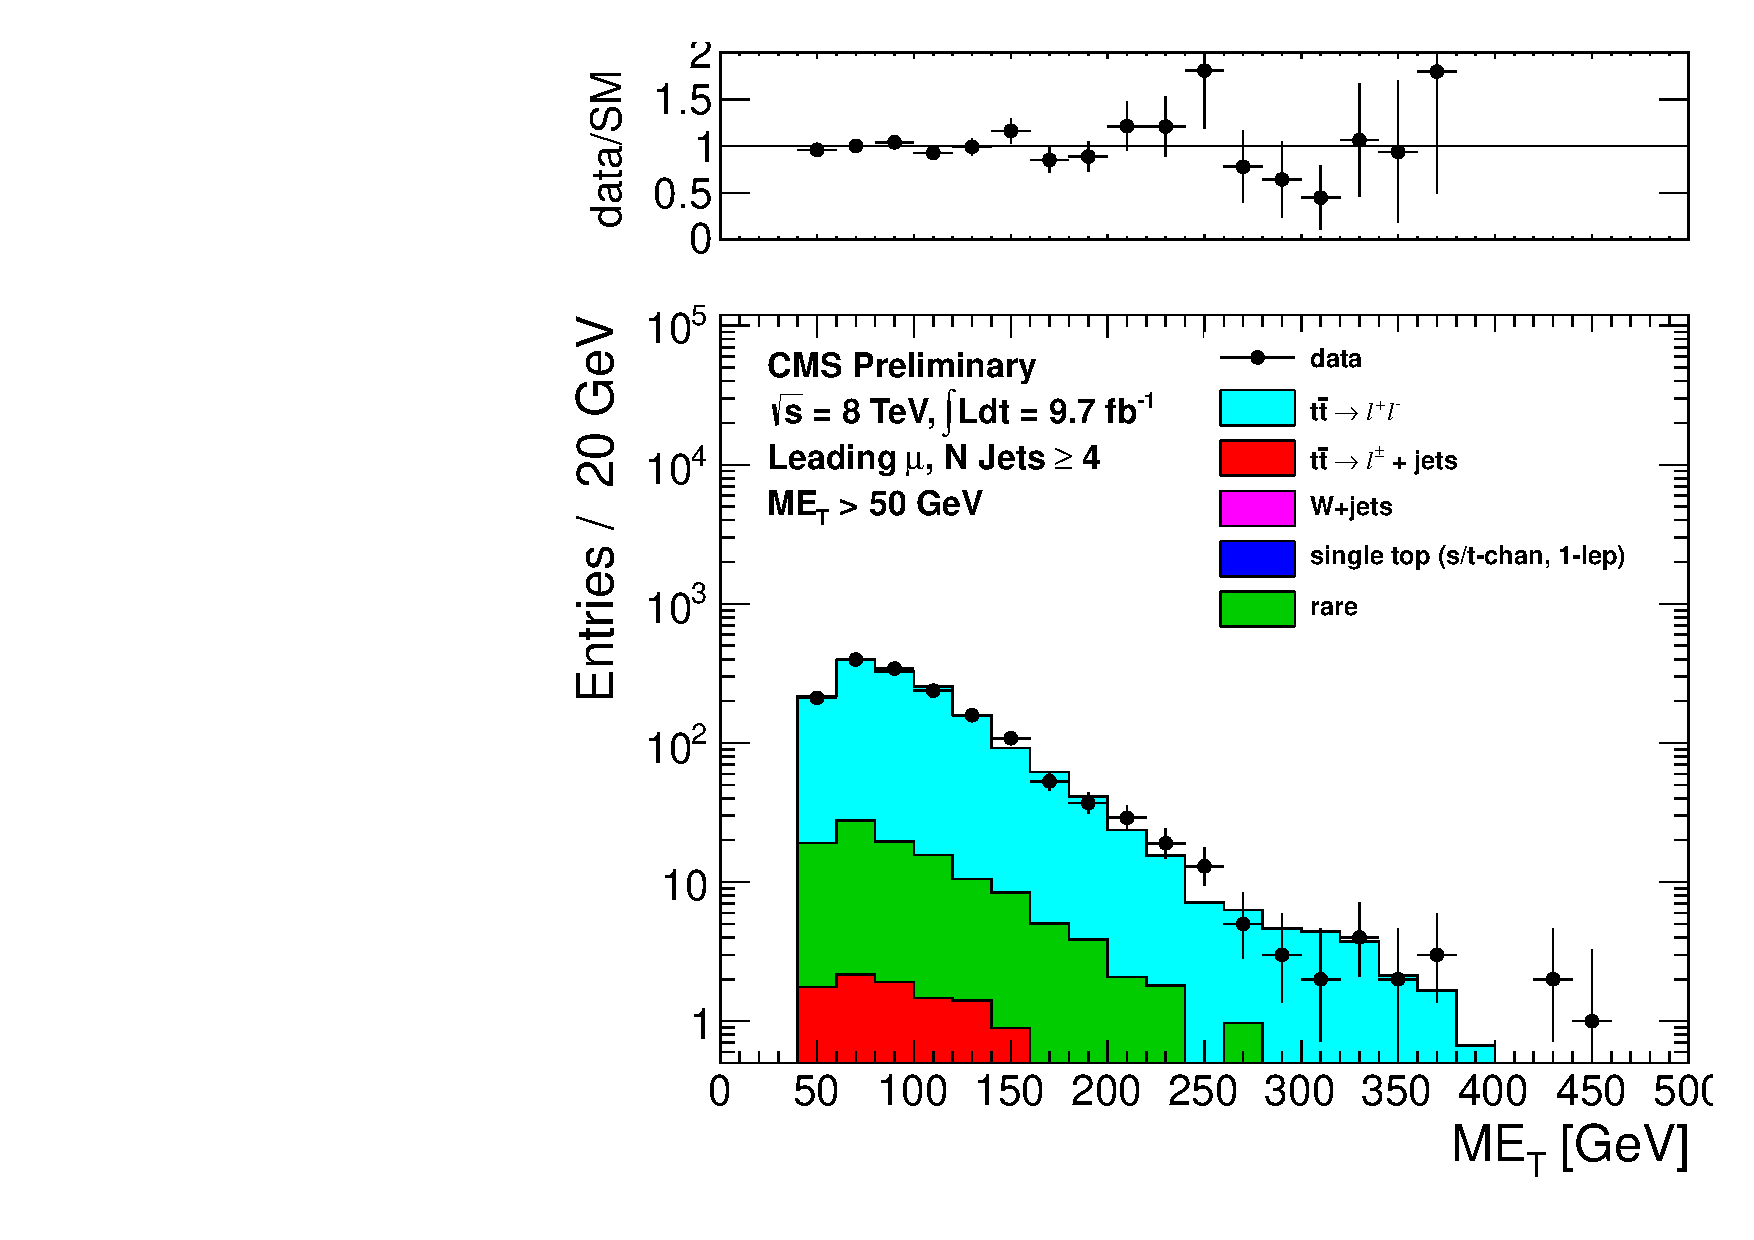
\includegraphics[width=0.5\linewidth]{plots/CR4plots/met_met50_leadmuo_nj4.pdf}%
        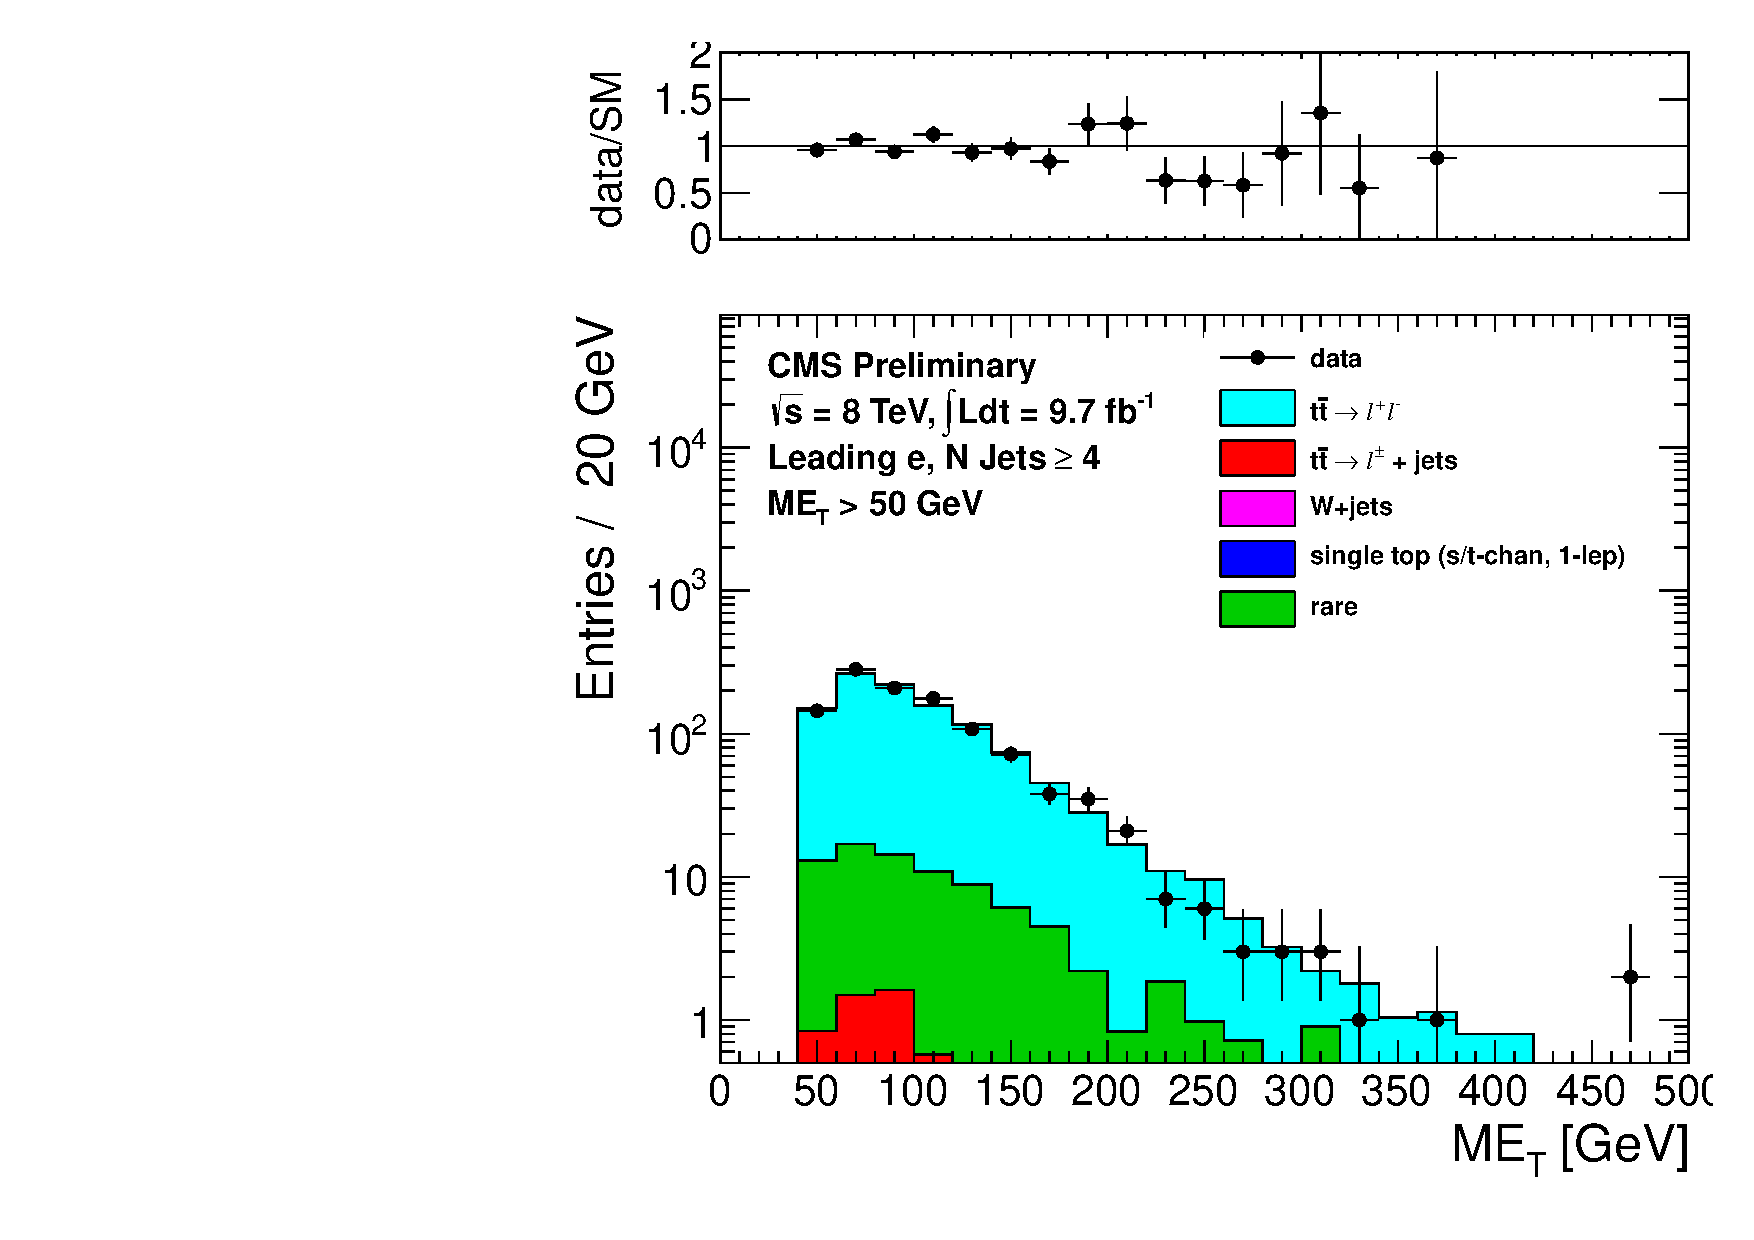
\includegraphics[width=0.5\linewidth]{plots/CR4plots/met_met50_leadele_nj4.pdf}
        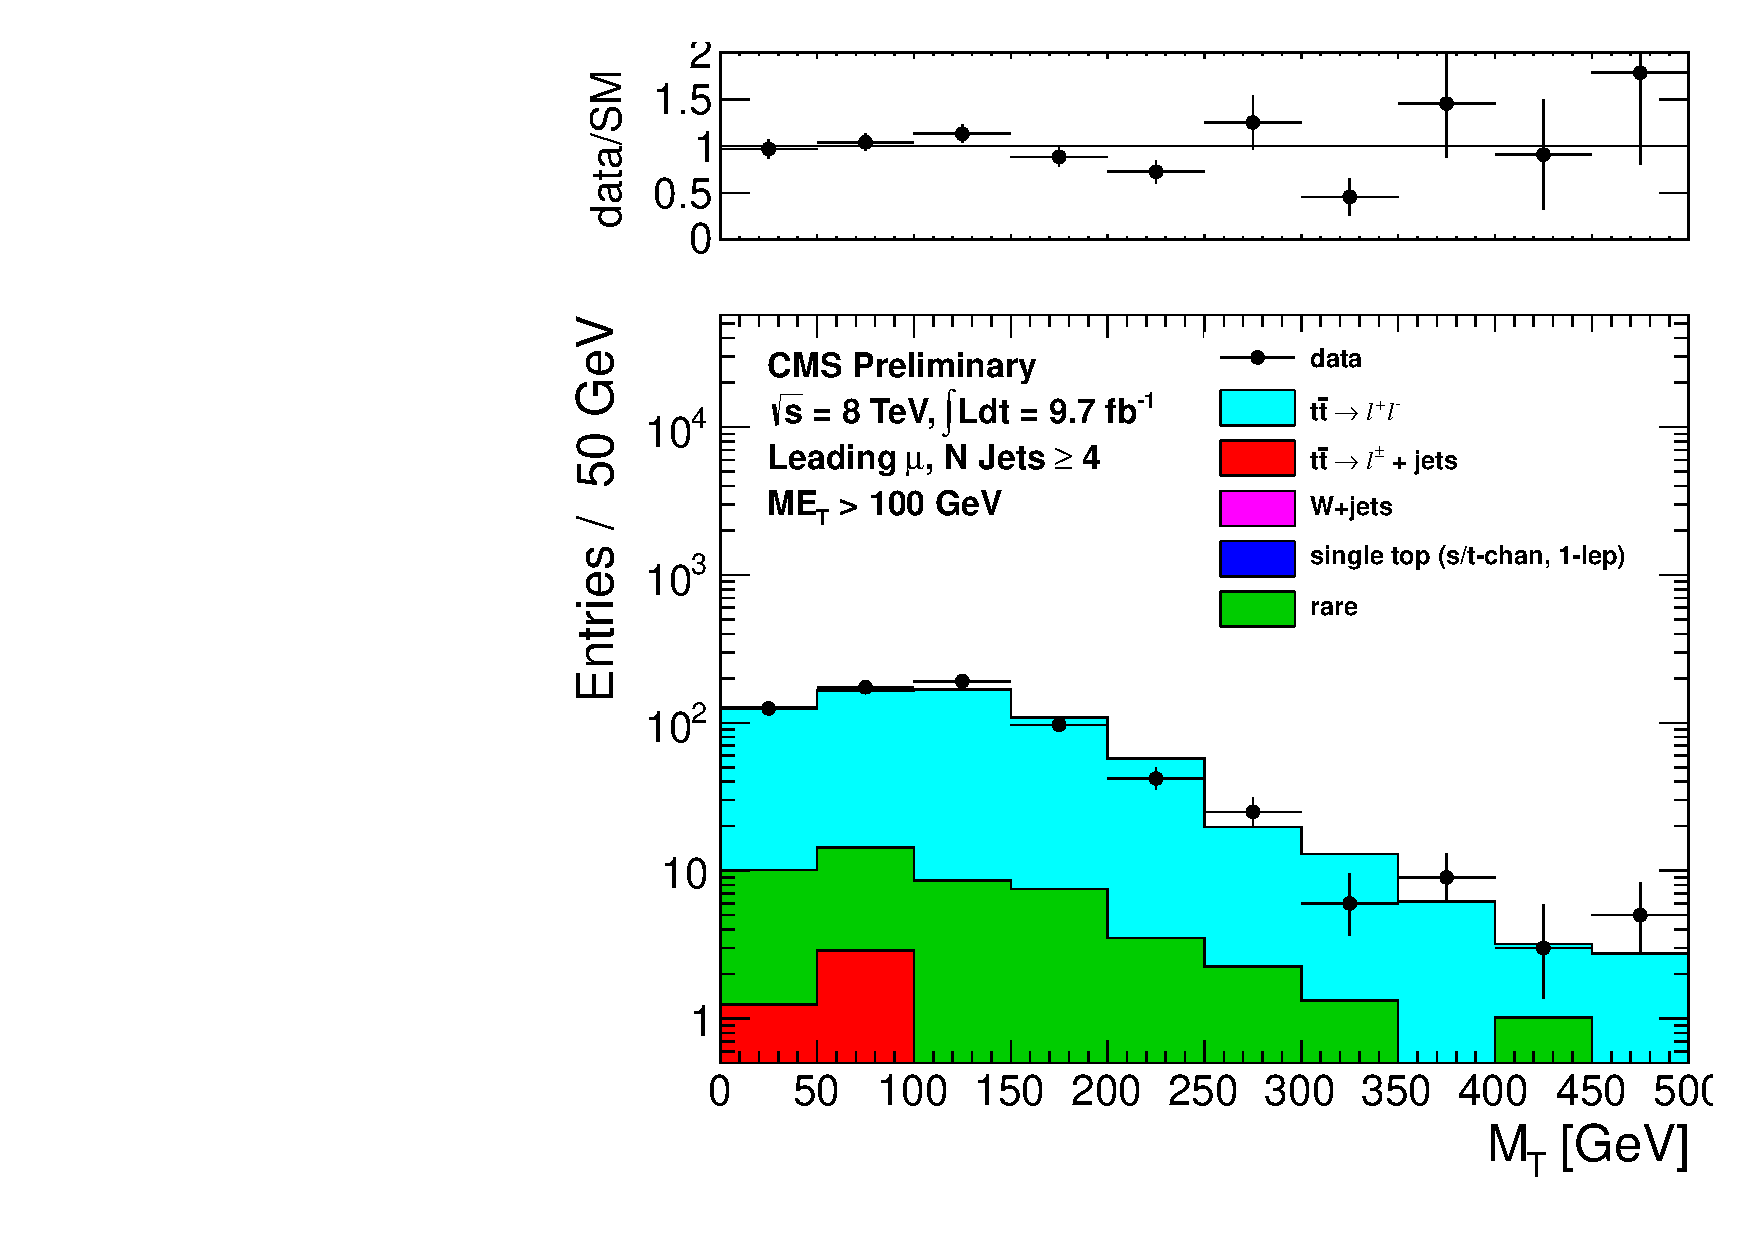
\includegraphics[width=0.5\linewidth]{plots/CR4plots/mt_met100_leadmuo_nj4.pdf}%
        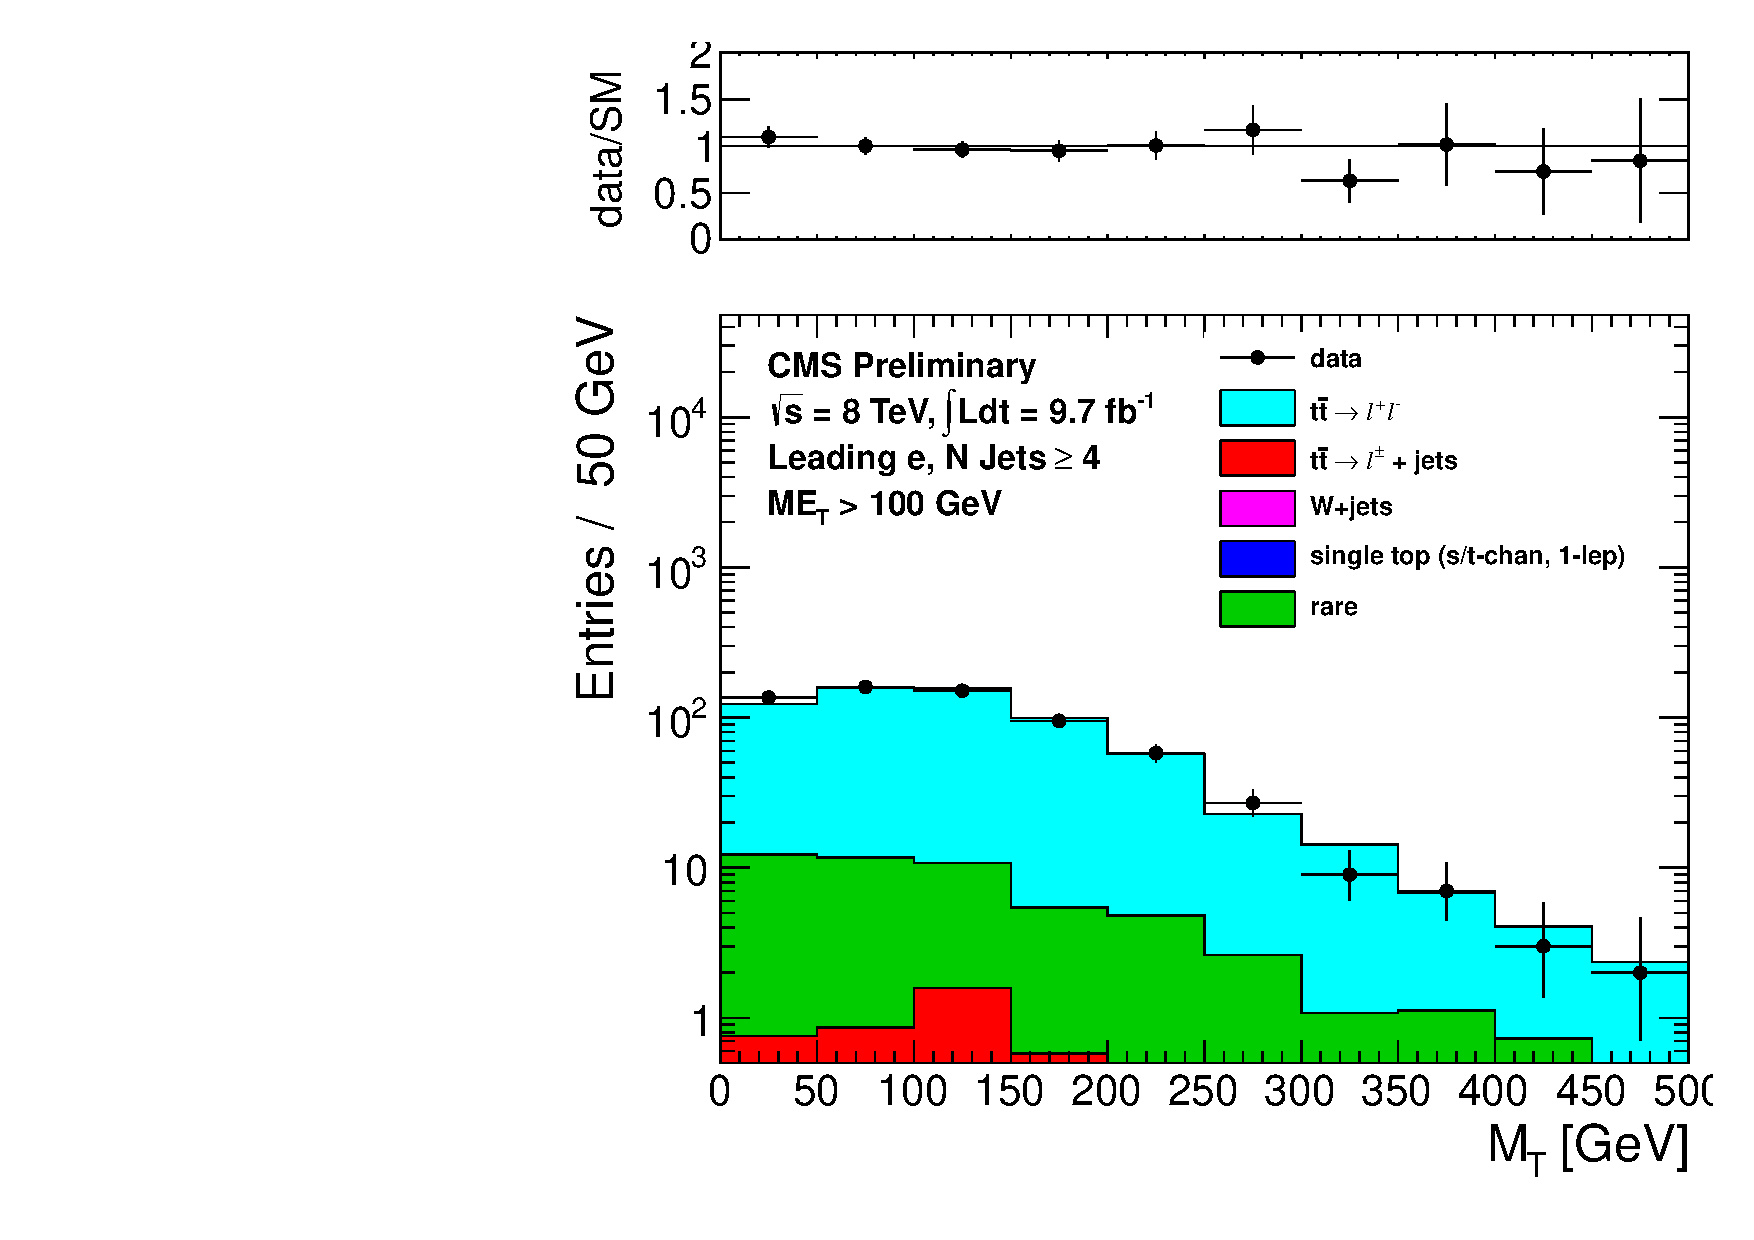
\includegraphics[width=0.5\linewidth]{plots/CR4plots/mt_met100_leadele_nj4.pdf}
    \caption{
      Comparison of the \met\ (top) and \mt\ for $\met>100$ (bottom) distributions in data vs. MC for events
      with a leading muon (left) and leading electron (right)
      satisfying the requirements of CR4. 
\label{fig:cr4met} 
}  
      \end{center}
\end{figure}

\begin{figure}[hbt]
  \begin{center}
        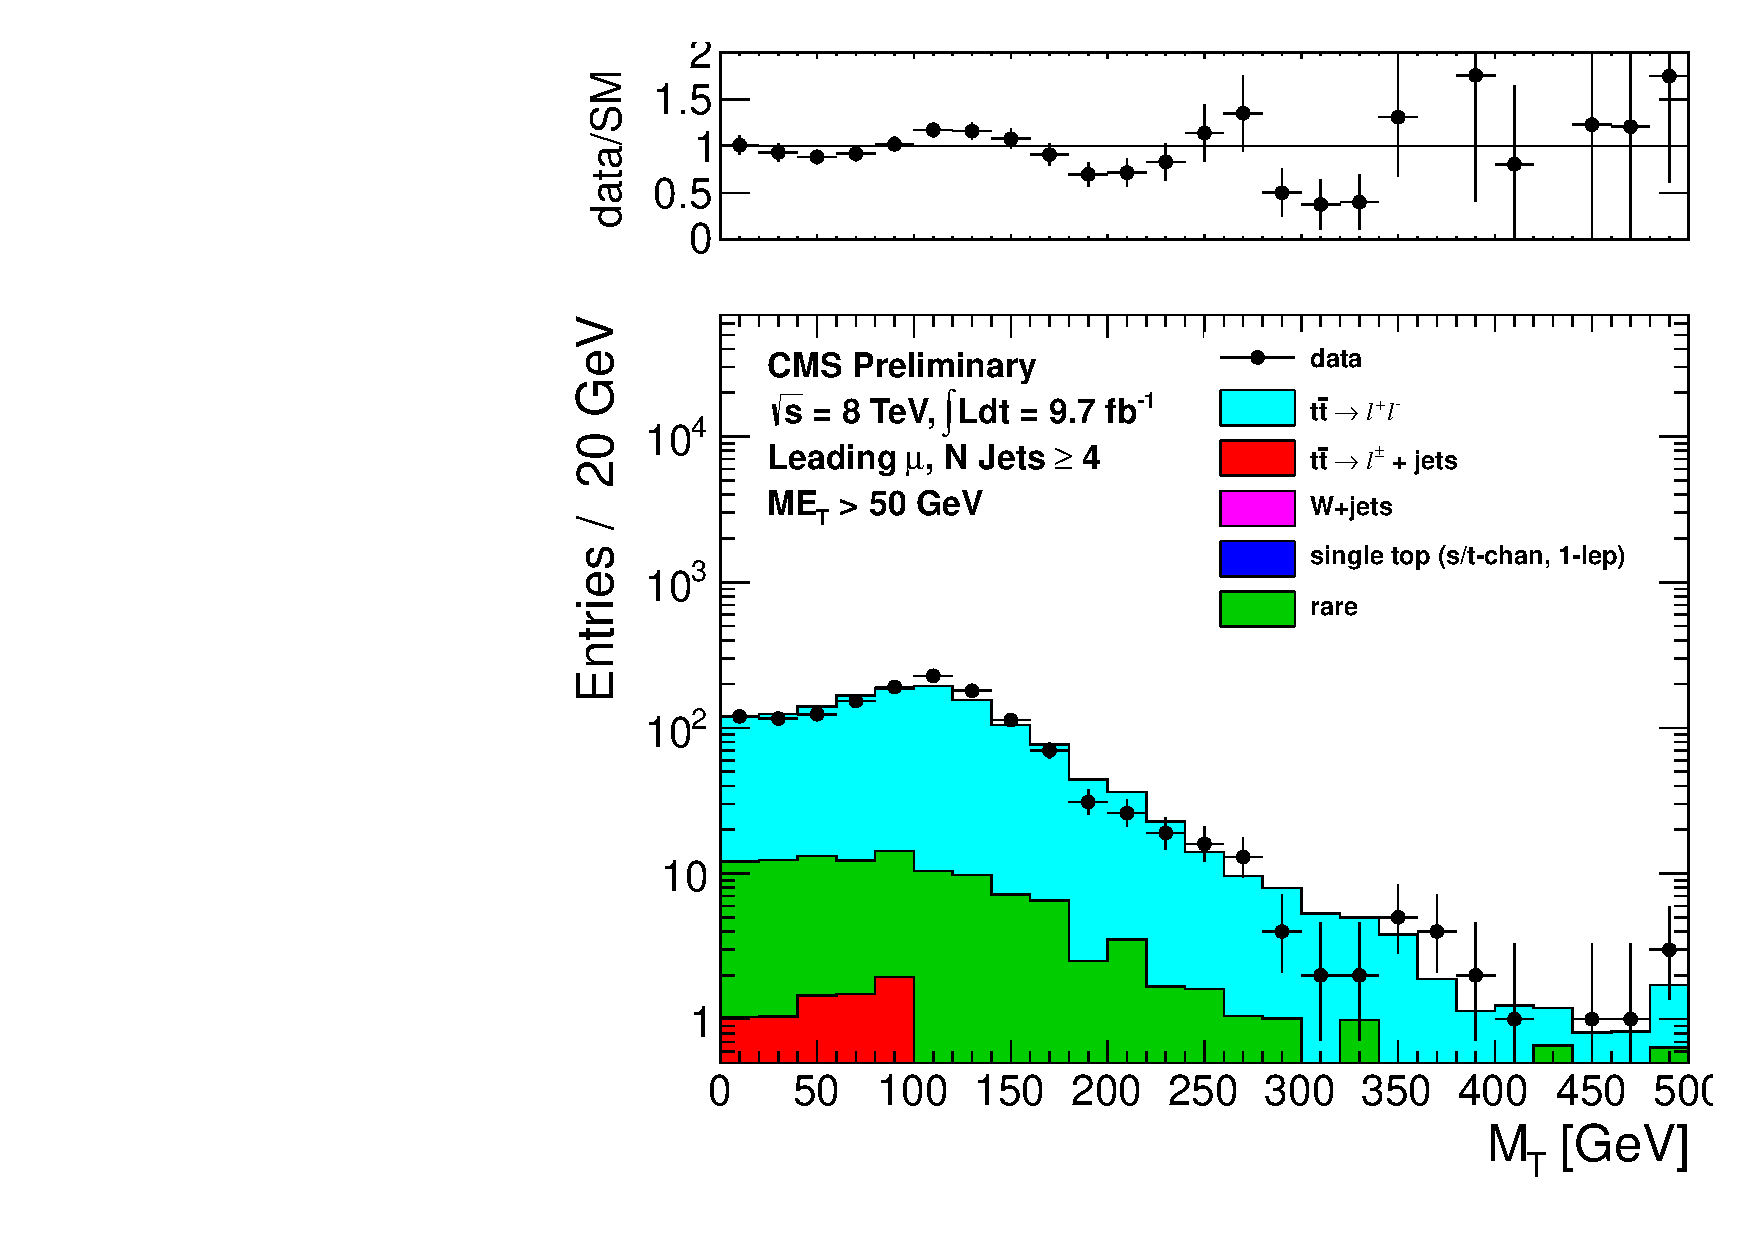
\includegraphics[width=0.5\linewidth]{plots/CR4plots/mt_met50_leadmuo_nj4.pdf}%
        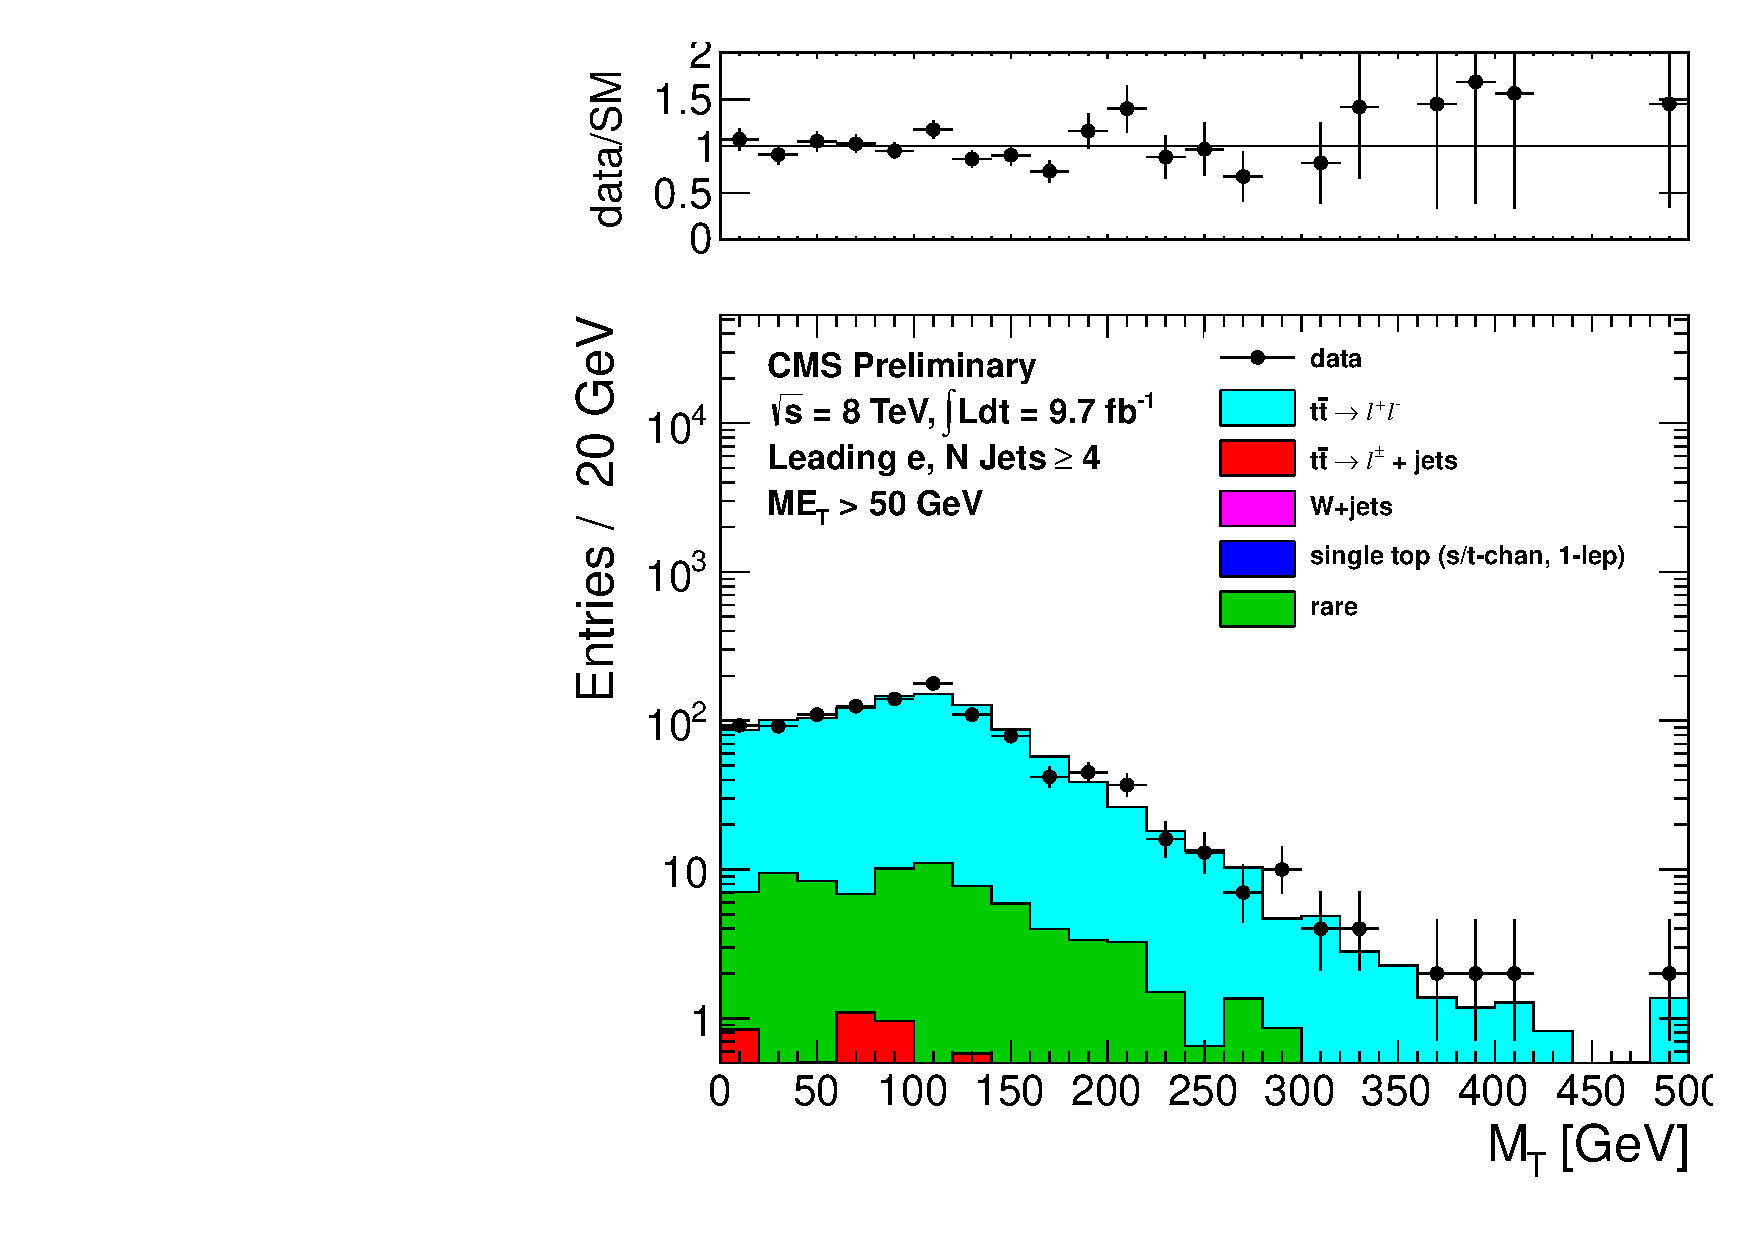
\includegraphics[width=0.5\linewidth]{plots/CR4plots/mt_met50_leadele_nj4.pdf}
        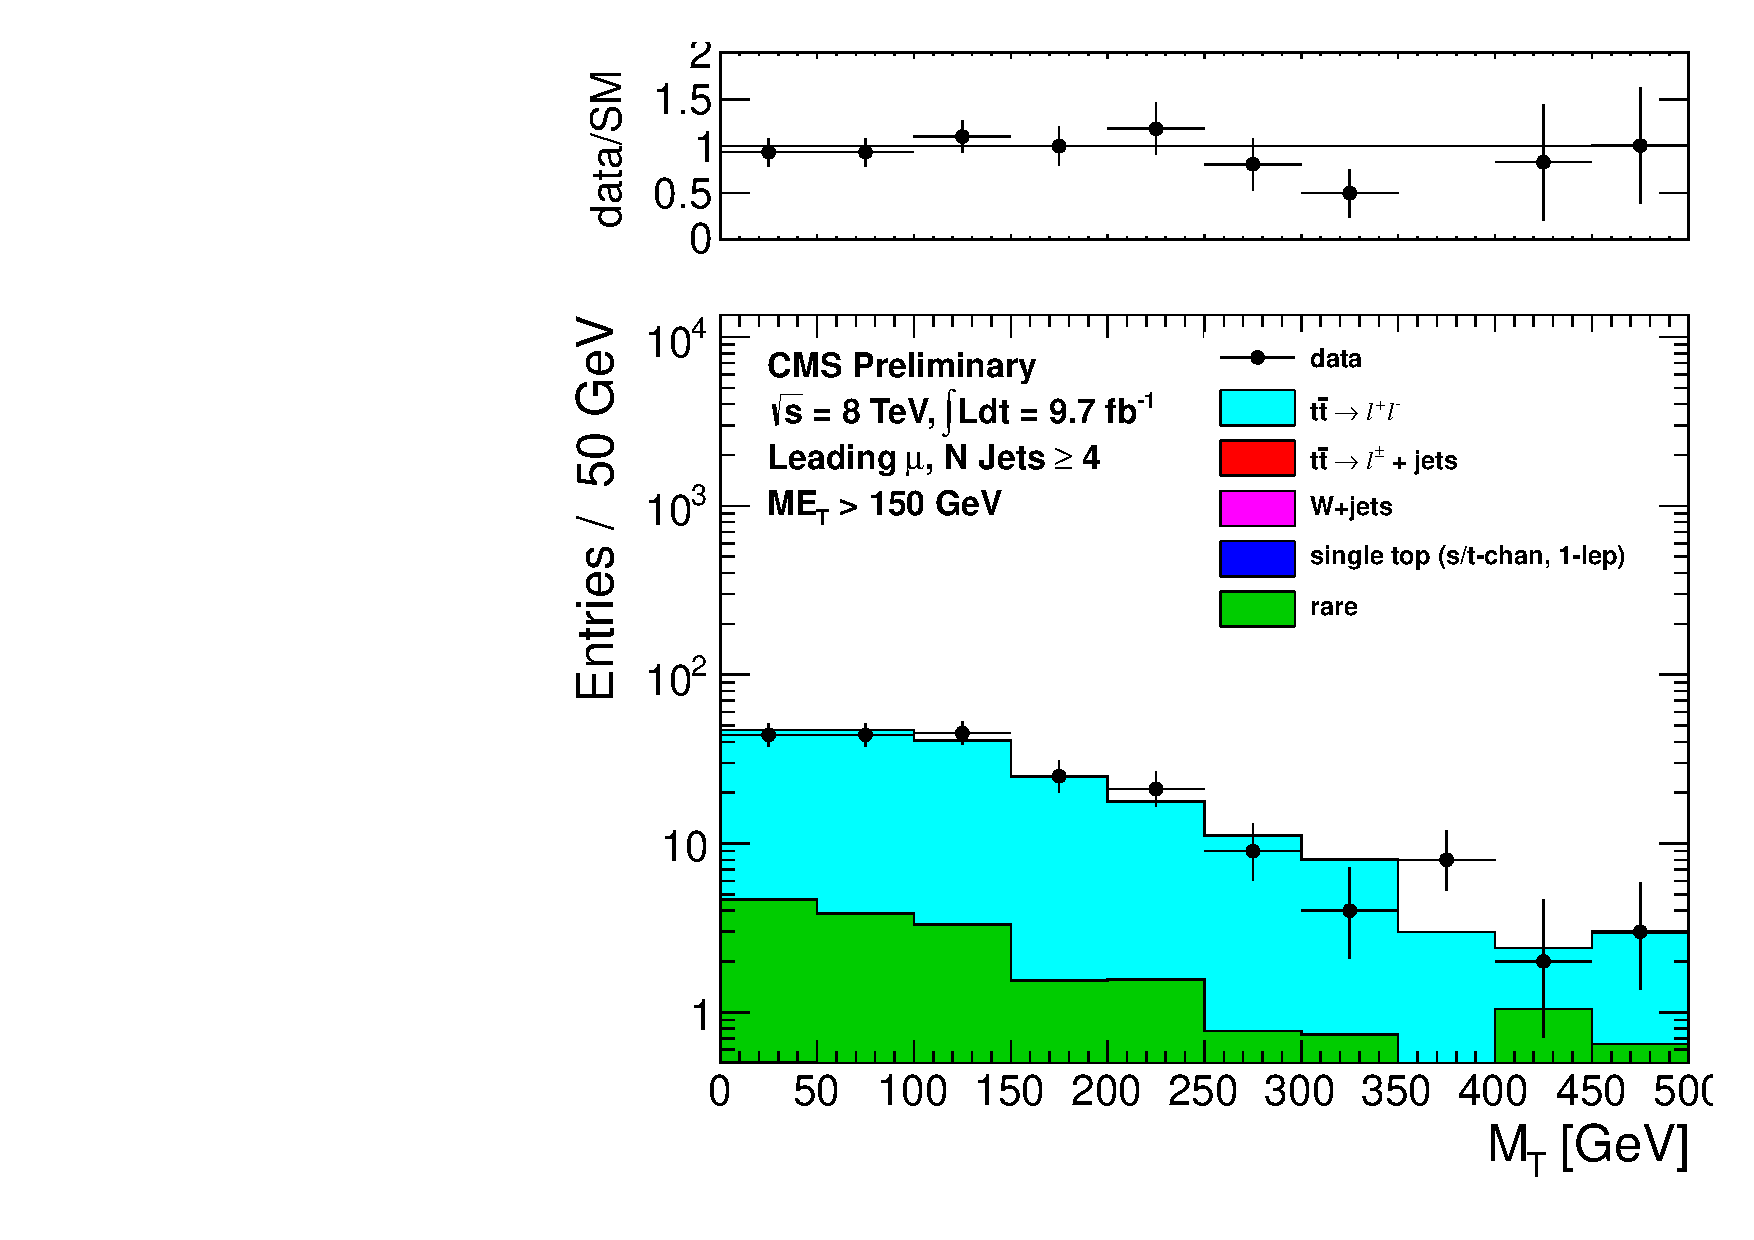
\includegraphics[width=0.5\linewidth]{plots/CR4plots/mt_met150_leadmuo_nj4.pdf}%
        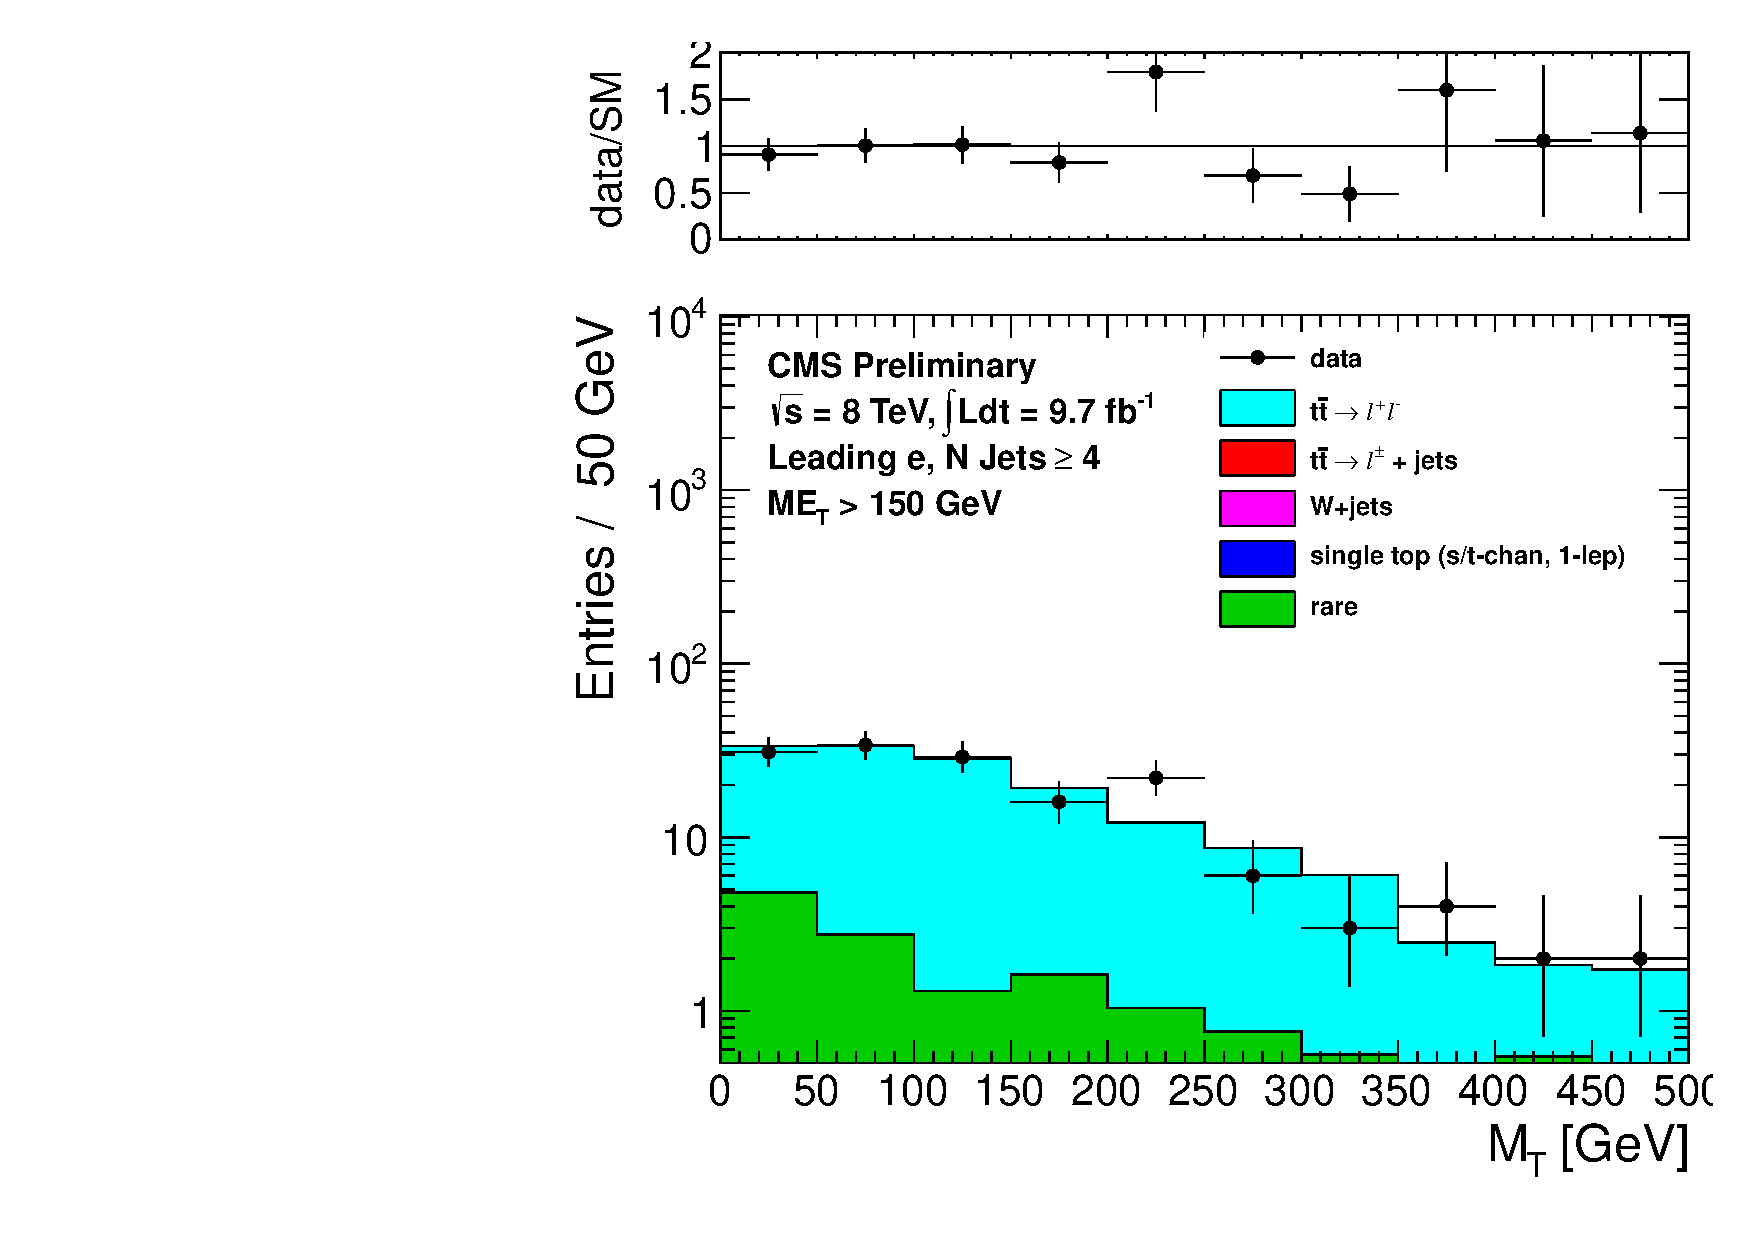
\includegraphics[width=0.5\linewidth]{plots/CR4plots/mt_met150_leadele_nj4.pdf}
        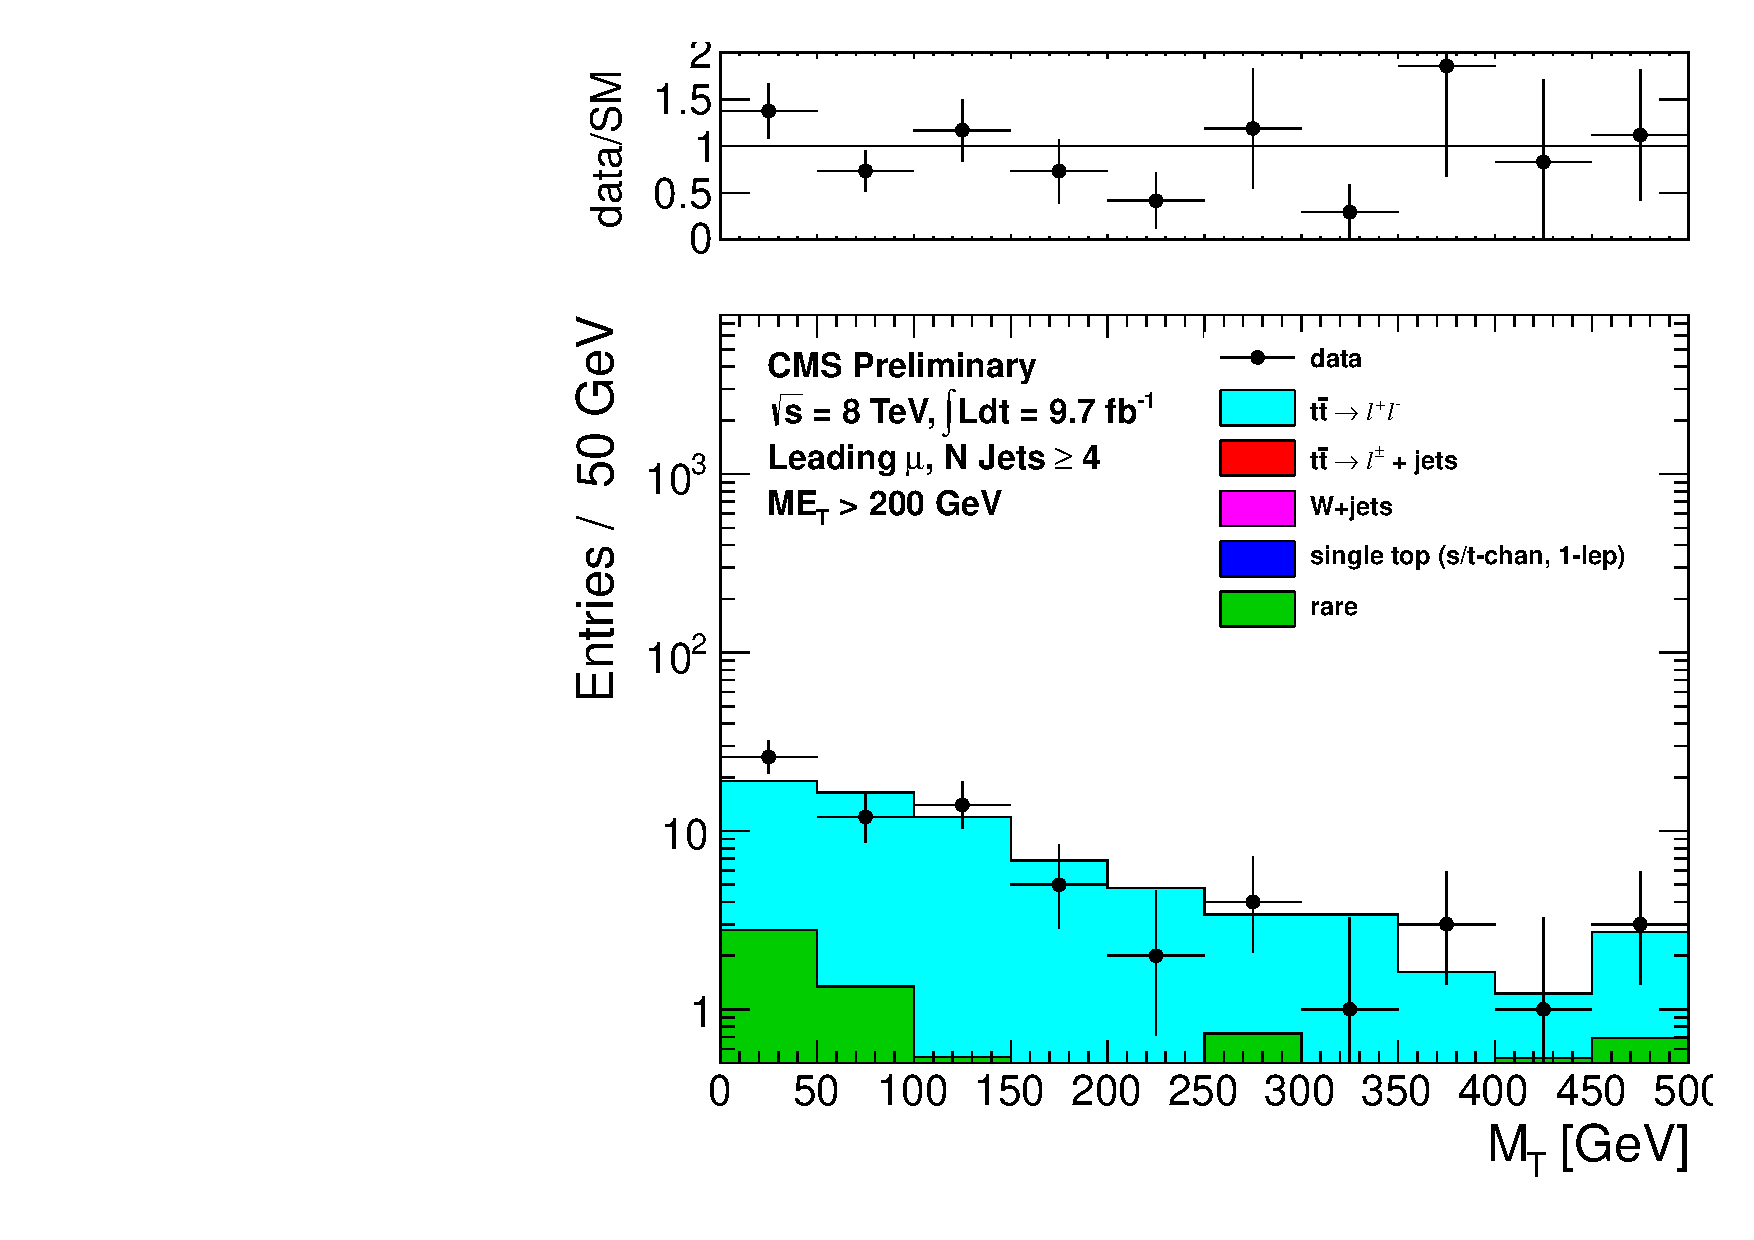
\includegraphics[width=0.5\linewidth]{plots/CR4plots/mt_met200_leadmuo_nj4.pdf}%
        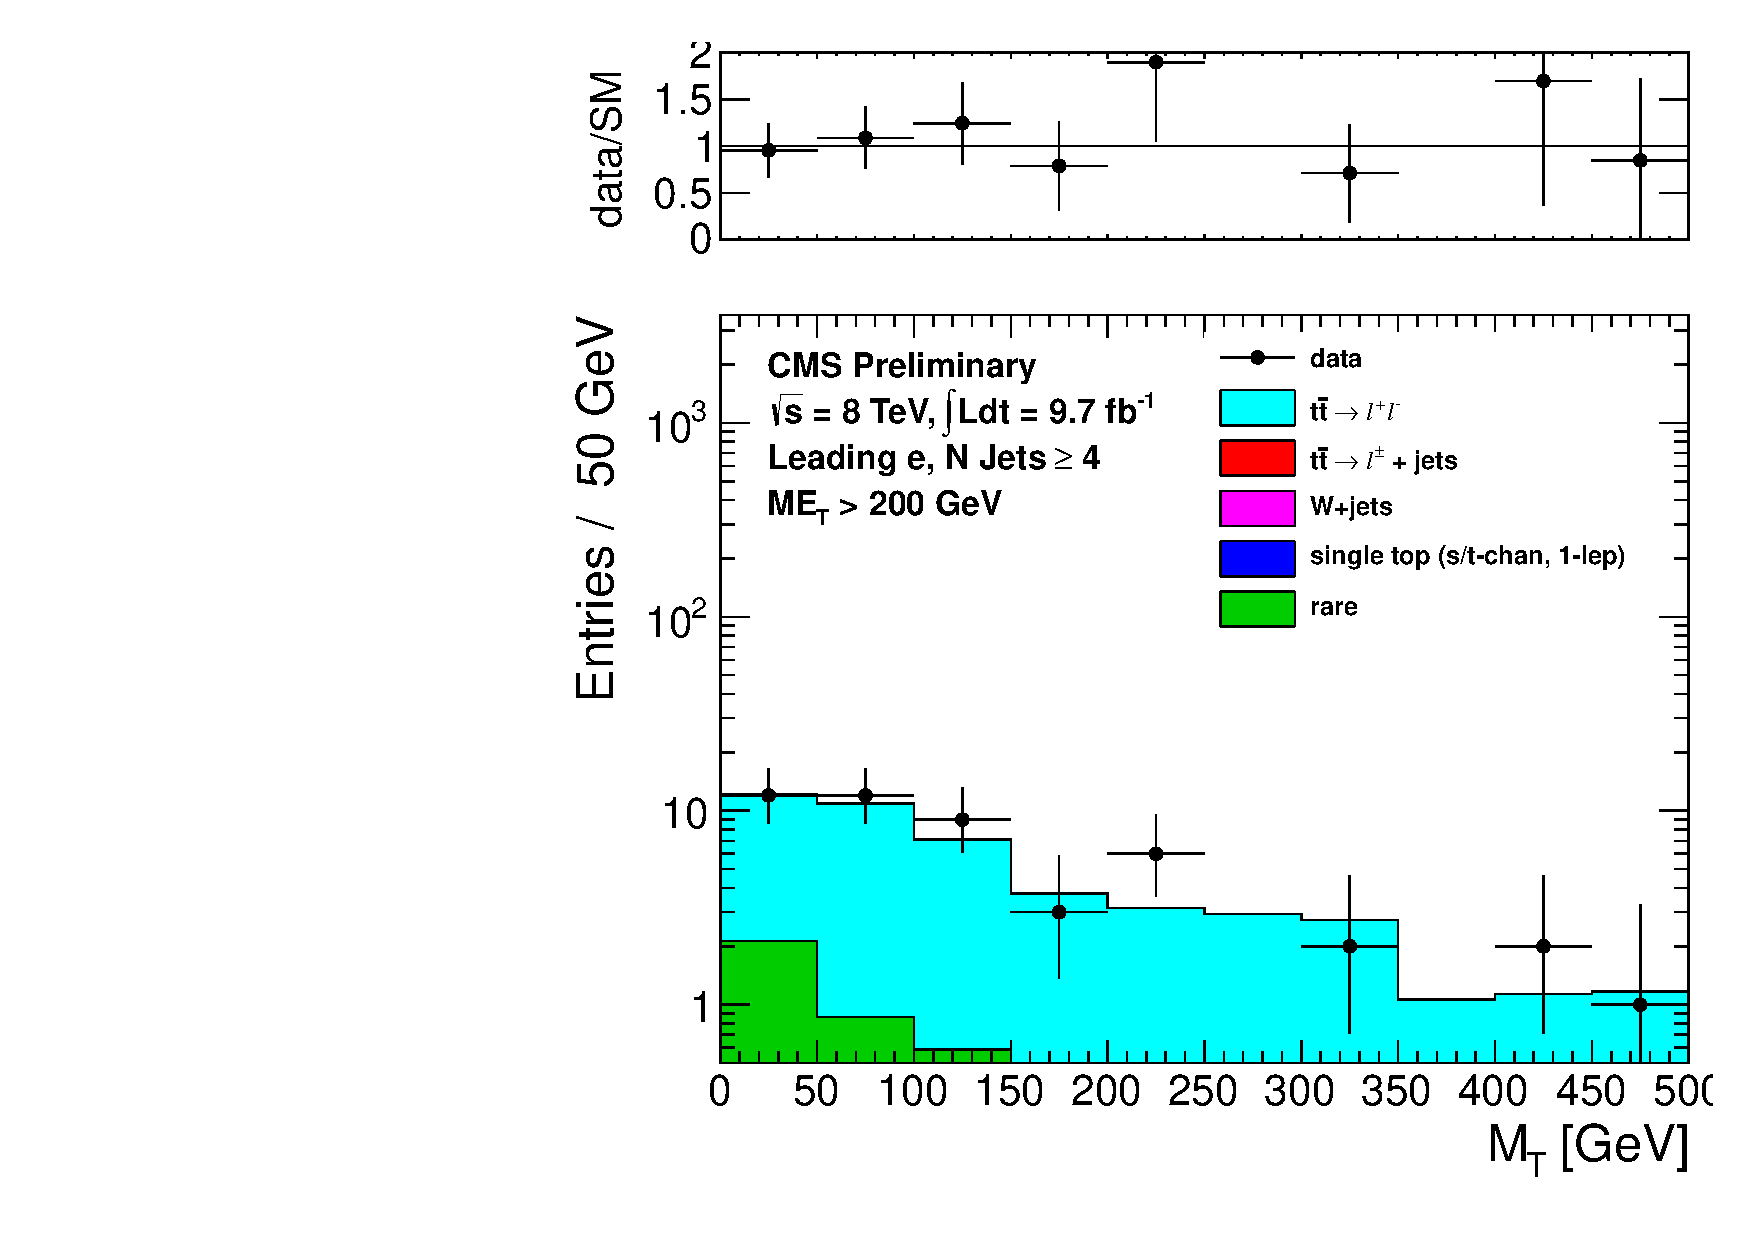
\includegraphics[width=0.5\linewidth]{plots/CR4plots/mt_met200_leadele_nj4.pdf}
    \caption{
      Comparison of the \mt\ distribution in data vs. MC for events
      with a leading muon (left) and leading electron (right)
      satisfying the requirements of CR4. The \met\ requirements used are
      50 GeV (top), 200 GeV (middle) and 250 GeV (bottom).
\label{fig:cr4mtrest} 
}  
      \end{center}
\end{figure}


\clearpage
